\documentclass[letterpaper, 10 pt, conference]{ieeeconf}  % Comment this line out if you need a4paper
%\documentclass[a4paper, 10pt, conference]{ieeeconf}      % Use this line for a4 paper
\IEEEoverridecommandlockouts                              % This command is only needed if 
                                                          % you want to use the \thanks command
\overrideIEEEmargins                                      % Needed to meet printer requirements.

\usepackage[pdftex]{graphicx}
\usepackage{algpseudocode}
\usepackage{subfigure}
\usepackage[noadjust]{cite}

\title{\LARGE \bf
  % Longitudinal Trajectory Planning and Tracking for Fixed-Path Autonomous Driving
  % Reactive Path Planning with Pedestrains for Autonomous Driving
  Reactive Trajectory Planning and Tracking for Pedestrian-Aware Autonomous Driving in Urban Environments
}

\author{
  Robert G. Cofield$^{1}$ and
  Rakesh Gupta$^{2}$
  \thanks{
    * This work was performed at Honda Research Institute USA.
  }
  \thanks{
    $^{1}$ Auburn University GAVLab, 1418 Wiggins Hall, Auburn, AL 36832. \textit{robertgcofield@gmail.com}
  }
  \thanks{
    $^{2}$ Honda Research Institute USA Inc, 375 Ravendale Drive, Mountain View, CA 94043. \textit{rgupta@hra.com}
  }
}

%%%%%%%%%%%%%%%%%%%%%%%%%%%%%%%%%%%%%%%%%%%%%%%%%%%%%%%%%%%%%%%%%%%%%%%%%%%%%%%%
%%%%%%%%%%%%%%%%%%%%%%%%%%%%%%%%%%%%%%%%%%%%%%%%%%%%%%%%%%%%%%%%%%%%%%%%%%%%%%%%
%%%%%%%%%%%%%%%%%%%%%%%%%%%%%%%%%%%%%%%%%%%%%%%%%%%%%%%%%%%%%%%%%%%%%%%%%%%%%%%%

\begin{document}

\maketitle
\thispagestyle{empty}
\pagestyle{empty}

%%%%%%%%%%%%%%%%%%%%%%%%%%%%%%%%%%%%%%%%%%%%%%%%%%%%%%%%%%%%%%%%%%%%%%%%%%%%%%%%
\begin{abstract}
In this paper, we address the problem of trajectory planning for an autonomous car for urban roads while reacting to the presence of pedestrians.
Past work limits jerk, velocities and acceleration for smooth trajectories, without considering reactive behaviors such as responding to pedestrians.
Other systems based on collision avoidance, plan paths around obstacles and pedestrians in unstructured environments.
In this paper, we present an integrated trajectory generation and tracking system for urban environments. Our system simultaneously considers constraints for smooth trajectory and updates the trajectory in real-time to react to pedestrians on the road. 

We present a novel online method for planning %longitudinal
trajectories to follow a given urban path while honoring traffic regulations such as stop signs at intersections. 
We update the trajectory to safely avoid pedestrians on the road by slowing down or stopping.
Our method has closed form solutions, runs at 20 Hz, and is efficient and reliable for use in online planning.
We have confirmed this with a test vehicle and pedestrians with over 100 hours of testing under driverless operation.

\end{abstract}
%%%%%%%%%%%%%%%%%%%%%%%%%%%%%%%%%%%%%%%%%%%%%%%%%%%%%%%%%%%%%%%%%%%%%%%%%%%%%%%%

%%%%%%%%%%%%%%%%%%%%%%%%%%%%%%%%%%%%%%%%%%%%%%%%%%%%%%%%%%%%%%%%%%%%%%%%%%%%%%%%
\section{Introduction} \label{sec:introduction}

%When planning trajectories for 
An autonomous ground vehicle operating on roadways, typically plans for trajectories with the goal of minimizing navigation time.
% "path-trajectory" is improper. "path-velocity" is used extensively in the literature.
It is common, to employ the path-velocity decomposition to separate the twin tasks of Path and Trajectory Planning, so that they can be run sequentially or in parallel.
% (i.e., path planning is performed prior to planning the speed that the vehicle will take along the chosen path).
Here {\it Path Planning} involves computation of the optimal path and {\it Trajectory Planning} involves the computation of a velocity profile appropriate for the scenario.

The set of possible paths to the destination is typically restricted
by constraints such as traversability and legally available travel lanes.
Trajectory computation for traveling on the path is often guided by passenger comfort. 
The intended speed, acceleration, and time derivatives of position are also subject to constraints.
These include legal speed limits, engine dynamics, desired side-slip limits, traction availability, and rollover risk.

For human passengers, it is widely believed that high levels of jerk (time derivative of acceleration) and high acceleration and velocity values are prime contributors to ride discomfort.
Lot of work has been performed on optimizing these constraints for highways and country roads ~\cite{ziegler14,bahram15,xu12,CHEB15CI}.
Similar work performed by Bianco et al \cite{GuarinoLoBianco2004,GuarinoLoBianco2005,Bianco2007,Bianco2009,GuarinoLoBianco2013} sets the travel time a priori and optimally minimizes ???what????? without hard limitations or direct jerk control.
Other work on optimizing these constraints on urban roads ~\cite{Rastelli14,Li15} doesn't consider reactive behaviors such as responding to pedestrians and other dynamic objects in the scene.

Many systems in the literature plan paths around pedestrians, stop for them, or produce a warning ~\cite{pradalier05,benenson06,gu14,mogelmose15,johnson13}. However, these systems do not work as part of an integrated system that navigates urban roads.
These systems also make the assumption that alternative paths around obstacles are available. Such an assumption may not always be valid in an urban scenario.
Planners that optimize human comfort by modifying the path to go around obstacles \cite{Villagra2012,Villagra2012a} do not feature stopping as a well-integrated behavior.
In this paper, we describe a trajectory generation system that satisfies the constraints for human comfort while being reactive to the presence of pedestrians on the road. We enforce hard upper limits on jerk without requiring that travel time is known for planning.
%Some work has been done for reacting to pedestrians such as by Singapore groups but it has been done at very low speeds (5 miles/hour).
%There has also been some work in simulating vehicles and modeling uncertainty, but pedestrians are less predictable than cars 
%and can appear suddenly on the road (when someone is jaywalking for example).

We would like our autonomous car to travel autonomously from start to destination while honoring traffic laws and avoiding pedestrians on the roadway.
%Desired behavior from the car includes following traffic laws at the intersections such as stop signs.
At stop signs, our autonomous car should stop and wait for an appropriate amount of time.
The car should also stop, slow down for pedestrians when appropriate.
It should react to pedestrians at the intersections as well as jay walking pedestrians.
Further, the pedestrians can be static or moving.
Pedestrians on the sidewalks should be ignored by the car.

\begin{figure}[tb]
  \centering
  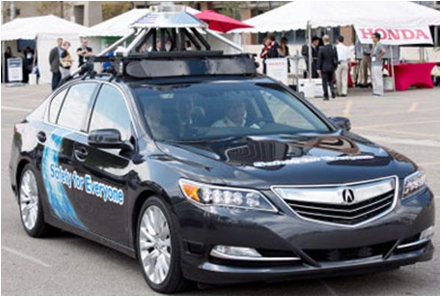
\includegraphics[width=0.7\columnwidth]{graphics/its_car.png}
  \caption{
    Showing car used in our experiments.
  }
  \label{fig:car}
\end{figure}

We present an autonomy framework for pedestrian-aware ground vehicles
with a novel method for planning longitudinal trajectories 
%(the time derivatives of position in the body-forward direction) 
along the desired path. %without requiring prior knowledge of travel time.
Our method segments the path using a set of kinematic or dynamic constraints.
Each segment is then planned sequentially by choosing a piecewise constant jerk profile.
We intelligently choose a jerk profile from a set of pre-solved profiles such that acceleration is continuous and within limits throughout the entire path.
The resultant trajectory plan is then sampled to provide a reference for real-time vehicle control. %, which is called trajectory tracking. In urban environments, modifying the vehicle's intended path is often not possible. 
% We are not doing control or tracking control. We're doing tracking.
%We revise the trajectory plan online to safely avoid pedestrians by slowing down or stopping. % when no alternative paths are available.

Section \ref{sec:systemarchirecture} describes the architecture of our system and 
other subsystems that interact with our system.
Section \ref{sec:pathmanager} describes the high-level Path Manager that calls the trajectory planner as necessary to 
exhibit reactive behavior and stop for pedestrians that may appear on the road.
Section \ref{sec:trajectoryplanning} describes trajectory planning, where we generate a trajectory that satisfies maximum velocity, acceleration and jerk constraints. 
%We explain how we pass through intersections, turns in the road and planned stops at the stop signs.
%We then describe extensions to trajectory planner that handle reactivity to pedestrians in the environment. 
Once the trajectory plan is formulated, we send the reference signal to the controllers that govern steering, braking, and engine speed.
This is the trajectory tracking and is discussed in Section \ref{sec:trajectorytracking},
followed by conclusions and future extensions.
% tracking

%%%%%%%%%%%%%%%%%%%%%%%%%%%%%%%%%%%%%%%%%%%%%%%%%%%%%%%%%%%%%%%%%%%%%%%%%%%%%%%%
%%%%%%%%%%%%%%%%%%%%%%%%%%%%%%%%%%%%%%%%%%%%%%%%%%%%%%%%%%%%%%%%%%%%%%%%%%%%%%%%

\section{System Architecture} \label{sec:systemarchirecture}

Our system architecture is shown in Figure \ref{fig:addreact}. We have three major components: a High-Level Planner, a Low-Level Planner, and a Software Controller.

The High-Level Planner is referred to as the {\it Path Manager}, and performs decision-making as well as governs operation of the low-level planner.
Its primary functions are:
\begin{enumerate}
  \item Stop the vehicle at stop signs and wait until the associated intersection is clear before continuing.
  \item Reactively reduce speed or stop altogether for pedestrians which pose a collision risk, then continue when they are clear.
  \item Govern the Trajectory Planner.
\end{enumerate}
The Low-Level Planner is also referred to as the {\it Trajectory Planner}, and is responsible for quantifying the actions dictated by the Path Manager.
Its primary functions are:
\begin{itemize}
  \item Compute medium-range trajectories for a given path.
  \item Revise trajectories to react to pedestrians.
  \item Sample the current trajectory for input to the controller.
\end{itemize}

The Software Controller governs engine speed, braking, and steering.
It takes as an input a trajectory sampled at 10 Hz spanning 2 seconds, beginning at the moment of data transmission.
This short-term trajectory is oriented in the vehicle body frame.
This paper focuses on the Path Manager (Sec. \ref{sec:pathmanager}) and the Trajectory Planner (Sec. \ref{sec:trajectoryplanning} \& Sec. \ref{sec:trajectorytracking}).


Beyond these major components, our system has four primary input components: Navigation Filtering, Pedestrian Detection, a Path Planner, and a Map.
% nav filter
For Navigation Filtering, we use an ADMA-G  commercial automotive GPS/INS system.
It receives RTK corrections via cell modem.
It outputs global position, global heading, body frame velocity and body frame acceleration to centimeter level accuracy.

\begin{figure}[tb]
  \centering
  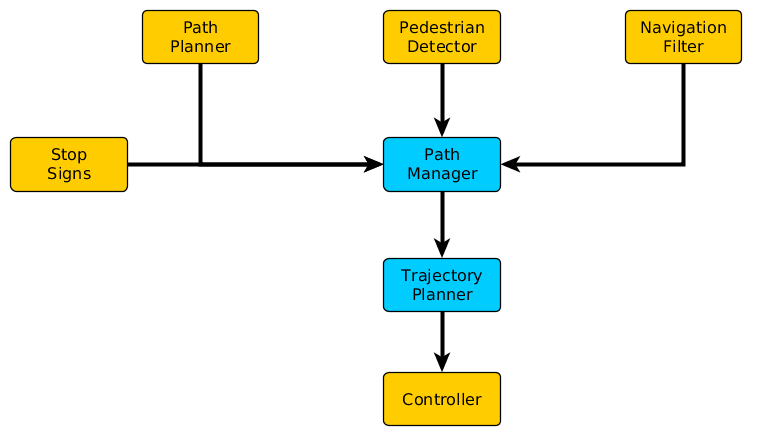
\includegraphics[width=1.0\columnwidth]{graphics/MissingReactionPiece2.png}
  \caption{
    Primary system components. The {\it Path Manager} and {\it Trajectory Planner} components (in blue) are presented herein.
  }
  \label{fig:addreact}
\end{figure}

Pedestrian Detection is performed via a camera and LiDAR system based on \cite{Gepperth2013,Gepperth2014}.
The pedestrian detector outputs a bounding box for each pedestrian as shown in Figure \ref{fig:ped}.
The pedestrian position is computed in the vehicle body frame, and subsequently transformed to the global frame to be related to the planned path.
Pedestrian detection algorithms are still in heavy development.
In order to make the algorithm robust to detection errors, it is designed under the assumption that pedestrian trajectory estimates and predictions are unavailable.
Furthermore, it is assumed that no unique identifier is available to differentiate one pedestrian from the other in a single epoch, or to correlate the same pedestrian between epochs.

\begin{figure}[tb]
  \centering
  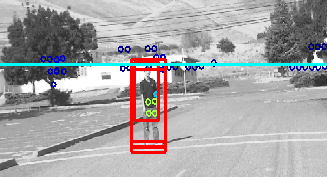
\includegraphics[width=0.5\columnwidth]{graphics/ped3.png}
  \caption{Showing detected pedestrian by the computer vision system
  \newline
  }
  \label{fig:ped}
\end{figure}

We assume access to a lane level Path Planner. For example, this can be a service similar to Google Maps except that it provides a lane level route instead of a road level route. 
We assume that the path planner operates independently from the trajectory planner and tracker.
%The destination is manually input into the system by the passengers.
Using the path planner, we obtain a path along lane centers from the vehicle's current location (computed by the navigation filter) to the user specified destination.
This plan is then output as a set of global waypoints.


%\begin{figure}[thpb]
%  \centering
%  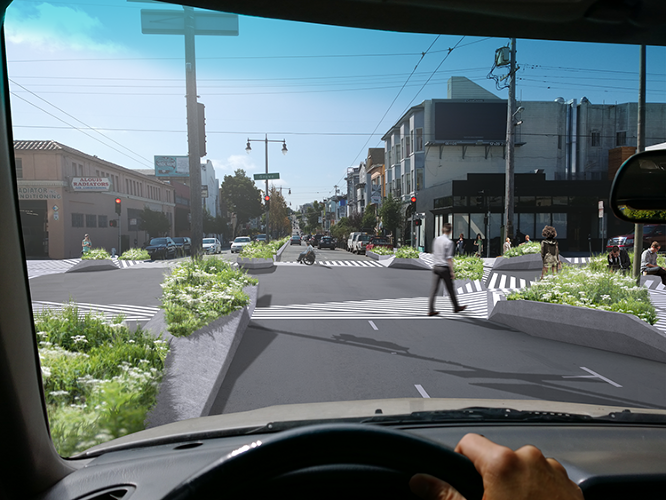
\includegraphics[width=1.0\columnwidth]{graphics/3023096-slide-c4carafter.png}
%  \caption{Pedestrain at the intersection}
%  \label{fig:ped2}
%\end{figure}

\begin{figure}[tb]
  \centering
  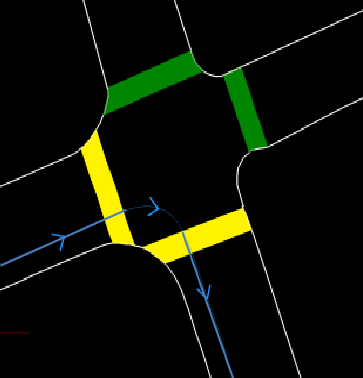
\includegraphics[width=0.3\columnwidth]{graphics/IntersectionCrosswalks.png}
  \caption{
    A car, with the blue line path, turning right at the intersection only needs to consider pedestrians in the zebra crossings shown in yellow.
    Pedestrians at the green crossings can be ignored unless they appear somewhere on the road.
  }
  \label{fig:intersect}
\end{figure}

We also assume a High-Resolution Digital Map with lane centers, stop signs, crosswalk geometry, and turning curves at intersections.
Our map provides the location of stop signs.
The plan waypoints corresponding to stop signs are then flagged for later processing.
We also have an In-Out Algorithm implemented via polygon intersection that can be used to ignore “safe” pedestrians
Pedestrians that are on sidewalks, behind planned stops, and off-path crosswalks as shown in Figure \ref{fig:intersect} can be considered {\it safe} and are ignored.
%This is done by searching the same map database used for path planning.
Remaining pedestrians pose collision risk and our vehicle needs to reactively slow down or stop for them.
%This is accomplished by sending stop message with pedestrian locations to the path manager.


%%%%%%%%%%%%%%%%%%%%%%%%%%%%%%%%%%%%%%%%%%%%%%%%%%%%%%%%%%%%%%%%%%%%%%%%%%%%%%%%
%%%%%%%%%%%%%%%%%%%%%%%%%%%%%%%%%%%%%%%%%%%%%%%%%%%%%%%%%%%%%%%%%%%%%%%%%%%%%%%%

\section{Path Manager} \label{sec:pathmanager}


The Path Manager performs trajectory planning over a sliding window within the full path with the sliding window moving with the vehicle.
As shown in Fig. \ref{fig:addreact}, a Path Planner passes paths into it as a 2D linestring.
It then breaks the path into sub-paths at each stop location which is known a priori, as shown in Fig. \ref{fig:subpathdivision}, and calls the Trajectory Planner for each sub-path in the path.

Prescribed initial and end conditions for the position, speed, and acceleration must be honored.
All planning is longitudinal; that is, speed profile generation is the primary focus. We assume that the control subsystem ensures that the vehicle follows the prescribed path.
This means that the desired trajectory plan may be mapped onto one dimension using curvilinear coordinates to significantly simplify the solution.
%We show how two dimensional constraints (specifically cornering speeds for this work) are expressed in one dimension to guide planning.
We express the 2D positions of the car (specifically cornering locations and speeds) in 1D $s$ coordinate system as described in Sec. \ref{sec:trajectorytracking} to guide planning.

Our Path Manager is implemented as a discrete state machine, depicted in Fig. \ref{fig:st}.
Each of the states is described below.

\begin{figure}[tb]
  \centering
  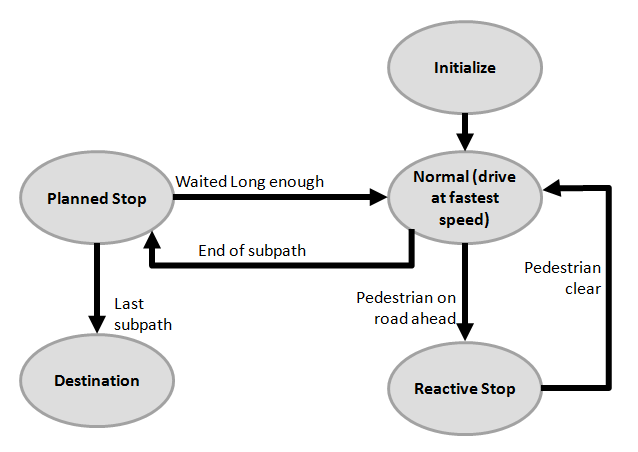
\includegraphics[width=0.6\columnwidth]{graphics/stgraph.PNG}
  \caption{State Transition Diagram for Path Manager. System transitions from NORMAL to PSTOP mode at each stop sign. In the presence of a pedestrian the system transitions to RSTOP.}
  \label{fig:st}
\end{figure}

In the absence of pedestrians, the path manager cycles between NORMAL and PSTOP states.
In NORMAL state, the path manager sends the first subpath to the trajectory planner, which then plans and executes it before coming to a stop at the end of the subpath.
In PSTOP mode, the path manager waits for a pre-set time duration before returning to NORMAL mode, where the next subpath is executed.
When pedestrians are present, the transition from PSTOP to NORMAL is delayed until there are no pedestrians detected in the range denoted by $\Delta s_{resume}$ as shown in Fig. \ref{fig:react}(c).

\begin{figure}[tb]
  \centering
  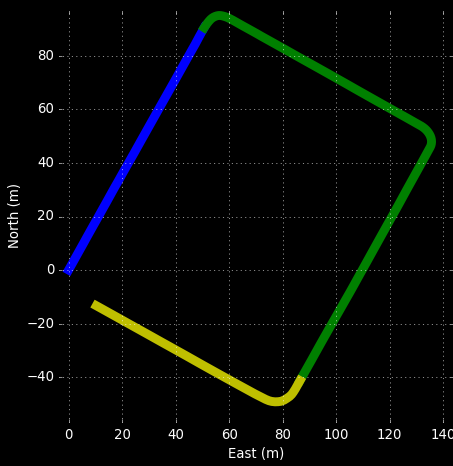
\includegraphics[width=0.5\columnwidth]{graphics/Subpaths.png}
  \caption{
    Dividing the path into sub-paths at stop signs.
    The Trajectory Planner is serially called for each sub-path shown in different color.
  }
  \label{fig:subpathdivision}
\end{figure}

All detected pedestrian locations are compared against the high-resolution digital map. Pedestrians that are off roadway are not considered.
Each pedestrian location is projected onto the 1D path in the same manner as described in Sec. \ref{sec:trajectorytracking}.
Pedestrians that are on a different subpath than the vehicle, or behind the vehicle are disregarded (i.e., $s_{ped} < s_{veh}$).
All the remaining pedestrians pose potential collision risks. However, only the closest pedestrian is considered for RSTOP.

The distinction between momentarily braking for a pedestrian that quickly leaves the roadway and coming to a full stop needs no separate logic.
They follow the same state transition, and since all trajectory plans are extremely smooth, riders are rarely aware that any change took place.
It should be noted that there is a brief waiting period before resuming NORMAL mode from RSTOP to ensure that no tracking errors occur in the pedestrian detection algorithm.

\begin{figure}[tb]
\centering
  \subfigure[In NORMAL mode, RSTOP is now triggered.]{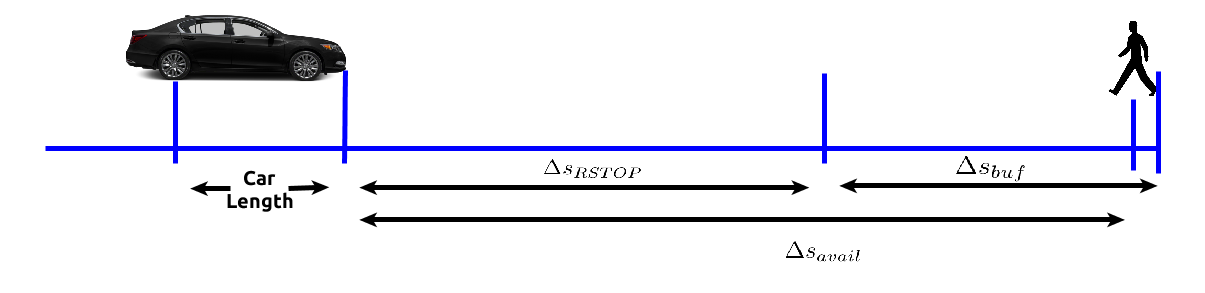
\includegraphics[width=1.0\columnwidth]{graphics/RSTOP_NORMAL_time_to_stop.png}}
  \\
  \subfigure[RSTOP diagram showing bounds for revising the RSTOP trajectory.]{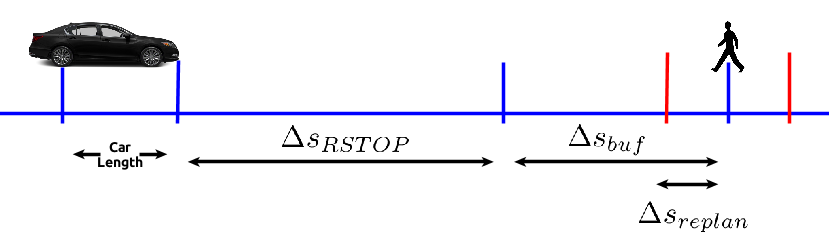
\includegraphics[width=1.0\columnwidth]{graphics/RSTOP_Replan.png}}
  \\
  \subfigure[PSTOP diagram showing bounds for reverting to NORMAL mode.]{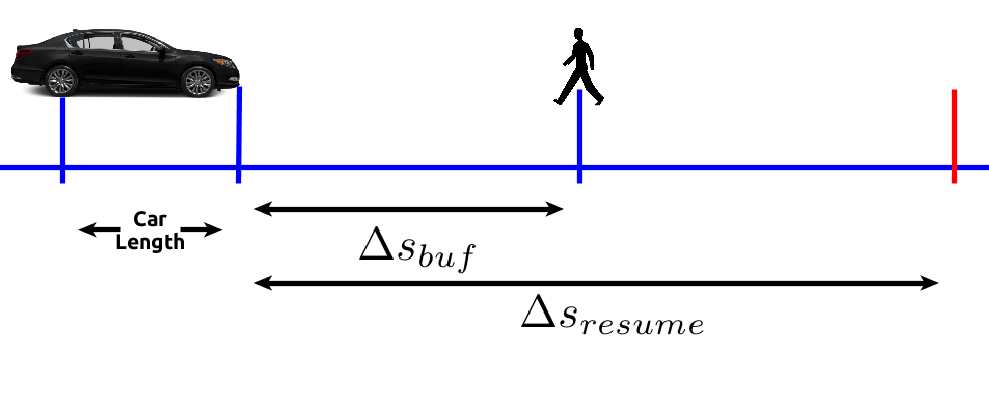
\includegraphics[width=1.0\columnwidth]{graphics/RSTOP_Resume.png}}
  \caption{Graphical representation of static and dynamic thresholds used to trigger state transitions.}
  \label{fig:react}
\end{figure}

When a pedestrian is detected, the nominal distance needed to stop, $\Delta s_{RSTOP}$, must be computed given the vehicle's current location, speed, and forward acceleration.
??????????? The procedure for doing this is the same as the procedure for planning the RSTOP trajectory with fewer steps, since the planning algorithm is quite efficient. ?????????? not clear

Note that a static buffer distance, $\Delta s_{buf}$ is added to ensure safety and comfort.
RSTOP is triggered when $\Delta s_{avail} <= \Delta s_{RSTOP} + \Delta s_{buf}$ and the actual available stopping distance $\Delta s_{avail} = s_{ped} - s_{veh}$ is computed.
Planning and executing the trajectory for coming to a halt is detailed in Sec. \ref{sec:reactivestoptrajectory}.

This procedure is repeated when the nearest pedestrian location changes by a value more than some static buffer $\Delta s_{replan} < \Delta s_{buf}$ compared to the location for which the current RSTOP planned.
$\Delta s_{replan}$ value is typically set to 1 meter.
Normal operation is resumed when the distance between the vehicle and the closest detected pedestrian satisfies $s_{ped} - s_{veh} > \Delta s_{resume} + \Delta s_{RSTOP}$. The static resume buffer should be set such that $\Delta s_{resume} > \Delta s_{buf} + \Delta s_{replan}$.
These quantities are depicted graphically in Fig. \ref{fig:react}.

%%%%%%%%%%%%%%%%%%%%%%%%%%%%%%%%%%%%%%%%%%%%%%%%%%%%%%%%%%%%%%%%%%%%%%%%%%%%%%%%
%%%%%%%%%%%%%%%%%%%%%%%%%%%%%%%%%%%%%%%%%%%%%%%%%%%%%%%%%%%%%%%%%%%%%%%%%%%%%%%%

\section{Trajectory Planning} \label{sec:trajectoryplanning}

The task of Trajectory Planning is to take a 1D set of waypoints from the Path Manager, and compute a series of constant jerk intervals for motion along the length of the path.
The resulting trajectory must be time optimal and satisfy all the constraints on speed, acceleration, and jerk.
%Elevation changes will not be addressed here.
Integrating piecewise constant jerk over time yields acceleration which is piecewise linear over time, a speed which is piecewise quadratic over time, and position which is piecewise cubic over time.

%%%%%%%%%%%%%%%%%%%%%%%%%%%%%%%%%%%%%%%%%%%%%%%%%%%%%%%%%%%%%%%%%%%%%%%%%%%%%%%%

\subsection{Path Segmentation} \label{sec:pathsegmentation}

In this section, we describe our approach to fitting appropriate jerk profiles to complex sub-paths. 
We first break each sub-path into segments with a simple shape.
Then each segment can be compared to a library of possible jerk profiles to find a good match.
Each segment is defined by the vector $\mathbf{b}  = [v_i, a_i, L, v_m, v_f]$, being initial speed, initial acceleration, the total distance, speed limit, and the final speed, respectively.
Additionally, the desired positive and negative acceleration $\mathbf{a}_m = [a^+_m , a^-_m]$ and the desired positive and negative jerk $\mathbf{j}_m = [j^+_m , j^-_m]$ must be defined for each segment.
A sub-path is then a set of $N$ segments, each of which is defined by a set of parameters $\mathbf{b}_{k}$, $\mathbf{a}_{m,k}$, and $\mathbf{j}_{m,k}$ where $k = 1, ..., N$ and can be solved individually in sequence.


The segmentation process proceeds as follows:
\begin{enumerate} \label{asdf}
  \item \emph{Ceiling Calculation}, where $v_m$, $\mathbf{a}_m$, and $\mathbf{j}_m$ 
%$initial/final speeds, speed limit, peak acceleration and jerk 
are found for every point in the given sub-path.
  \item \emph{Clustering}, in which sub-path points are grouped sequentially and the segment boundaries are determined.
  \item \emph{Consolidation}, in which a single $\mathbf{b}$, $\mathbf{a}_m$, and $\mathbf{j}_m$ is selected for each segment.
\end{enumerate}
After these steps are completed, the process for fitting jerk profiles described in next sub-section is applied to each of the segments to generate a plan of jerk vs. time.

The {\it Ceiling Calculation} is a minimax problem.
Each of the 9 scalars in $\mathbf{b}$, $\mathbf{a}_m$, and $\mathbf{j}_m$ is a minimum of several maxima computed from an arbitrary set of constraints.
For instance, acceleration constraints may include a set of limits derived from friction coefficients at every point along the sub-path.

% How we actually did this.
For the purposes of developing a simple example application, two constraints will be used for $v_{m}$: legal speed limit $SL$ and lateral acceleration limit $a_{B,y}^{max}$. 
Lateral acceleration constraints are translated into longitudinal speed constraints using the approximation 
%\textbf{ RG: using centrifugal  force relationship ????} 
$v_{m,w}(a_{B,y}) = \sqrt{a_{B,y}^{max}/\kappa_{w}}$ for $w = 1, ..., W$, where $W$ is the number of waypoints in the sub-path.
The value $\kappa_{k_P}$ denotes the path curvature at each point.
For each sub-path point, the value $v_{m,w}(a_{B,y}^{max})$ denotes the speed necessary to obtain the limit lateral acceleration, denoted by $a^{max}_{B,y}$.

This information is used to choose the segment boundaries in the {\it Clustering} step.
Any clustering algorithm may be used here, and a prudent choice of segment boundaries is arguably one of the most critical pieces of trajectory planning process.
We choose a simple univariate heuristic which identifies curves in the roadway using only the speed ceiling.
Each time $v_{m,w} < SL$ becomes true, a curve is beginning, and a segment boundary is drawn.
Each time $v_{m,w} = SL$ is once again true, the current curve has ended, and another segment boundary is drawn.

Figure \ref{fig:1Dto2DandSegmentation} shows the result of this Clustering algorithm. 
We start with a sub-path which is similar in structure to the sub-path between the stop signs in Fig. \ref{fig:subpathdivision}. This sub-path is broken up into five segments as shown in Fig. \ref{fig:1Dto2DandSegmentationa}, three shown in blue corresponding to straight line part of the sub-path and two shown in red corresponding to turns in the sub-path. As shown in Fig \ref{fig:1Dto2DandSegmentationb} we use the speed limit of 11.1 m/sec for the straight line segments and 3.0 m/sec for the turn segments to determine the segment boundaries. 
 
\begin{figure}[thpb]
  \centering
  \subfigure[
    The result of dividing a single sub-path into separate segments.
    The clustering algorithm used here sets segments boundaries before and after curves.
    The sub-path segments in red indicate areas where the longitudinal speed required to adhere to lateral acceleration limits is below the legal speed limit of 11.1 m/s (25 mi/hr).
  ]{
  \label{fig:1Dto2DandSegmentationa}
    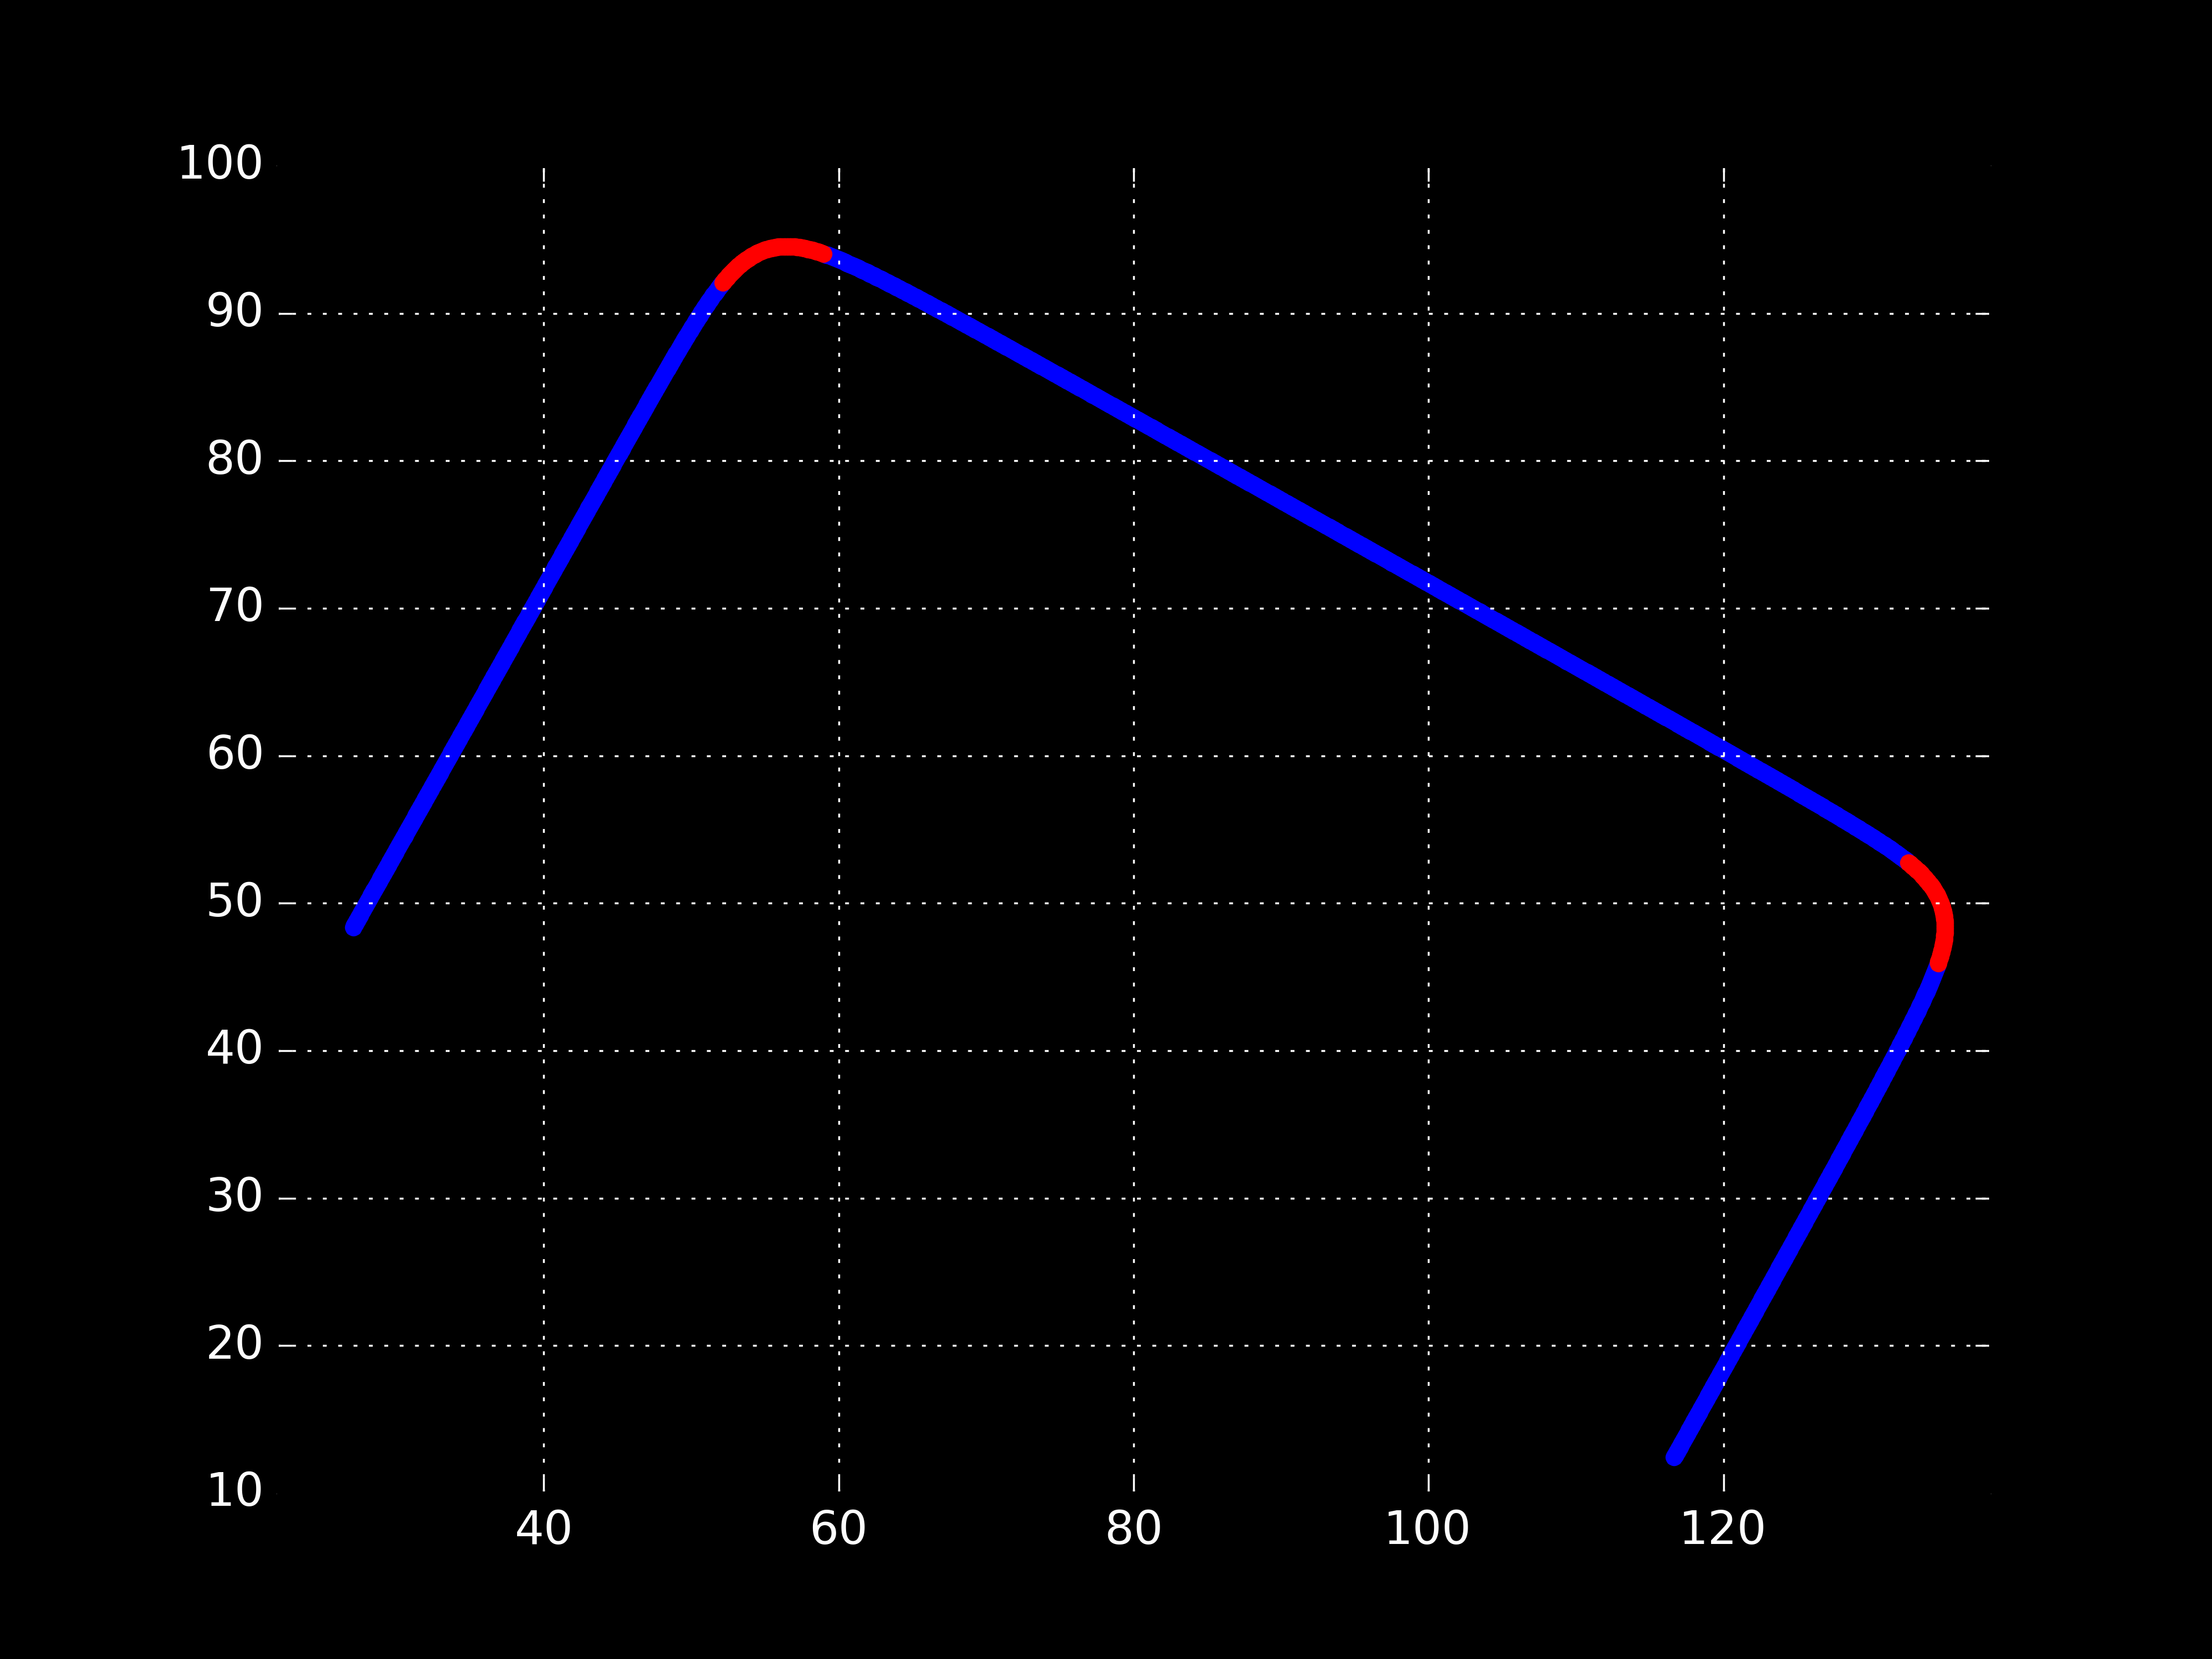
\includegraphics[width=0.8\columnwidth]{graphics/course_highlighted_turns.png}
  }
  \\
  \subfigure[
    An example of how the sub-path's segment boundaries are determined, as well as how $v_m$ is consolidated to determine the speed ceiling for each segment.
    The x-axis corresponds to distance along the subpath above.
    The legal speed limit of 11.1 m/s (25 mi/hr) is shown in cyan.
    The longitudinal speed required to adhere to lateral acceleration limits is shown in red.
    The resultant speed ceiling is shown in blue.
  ]{
  \label{fig:1Dto2DandSegmentationb}
  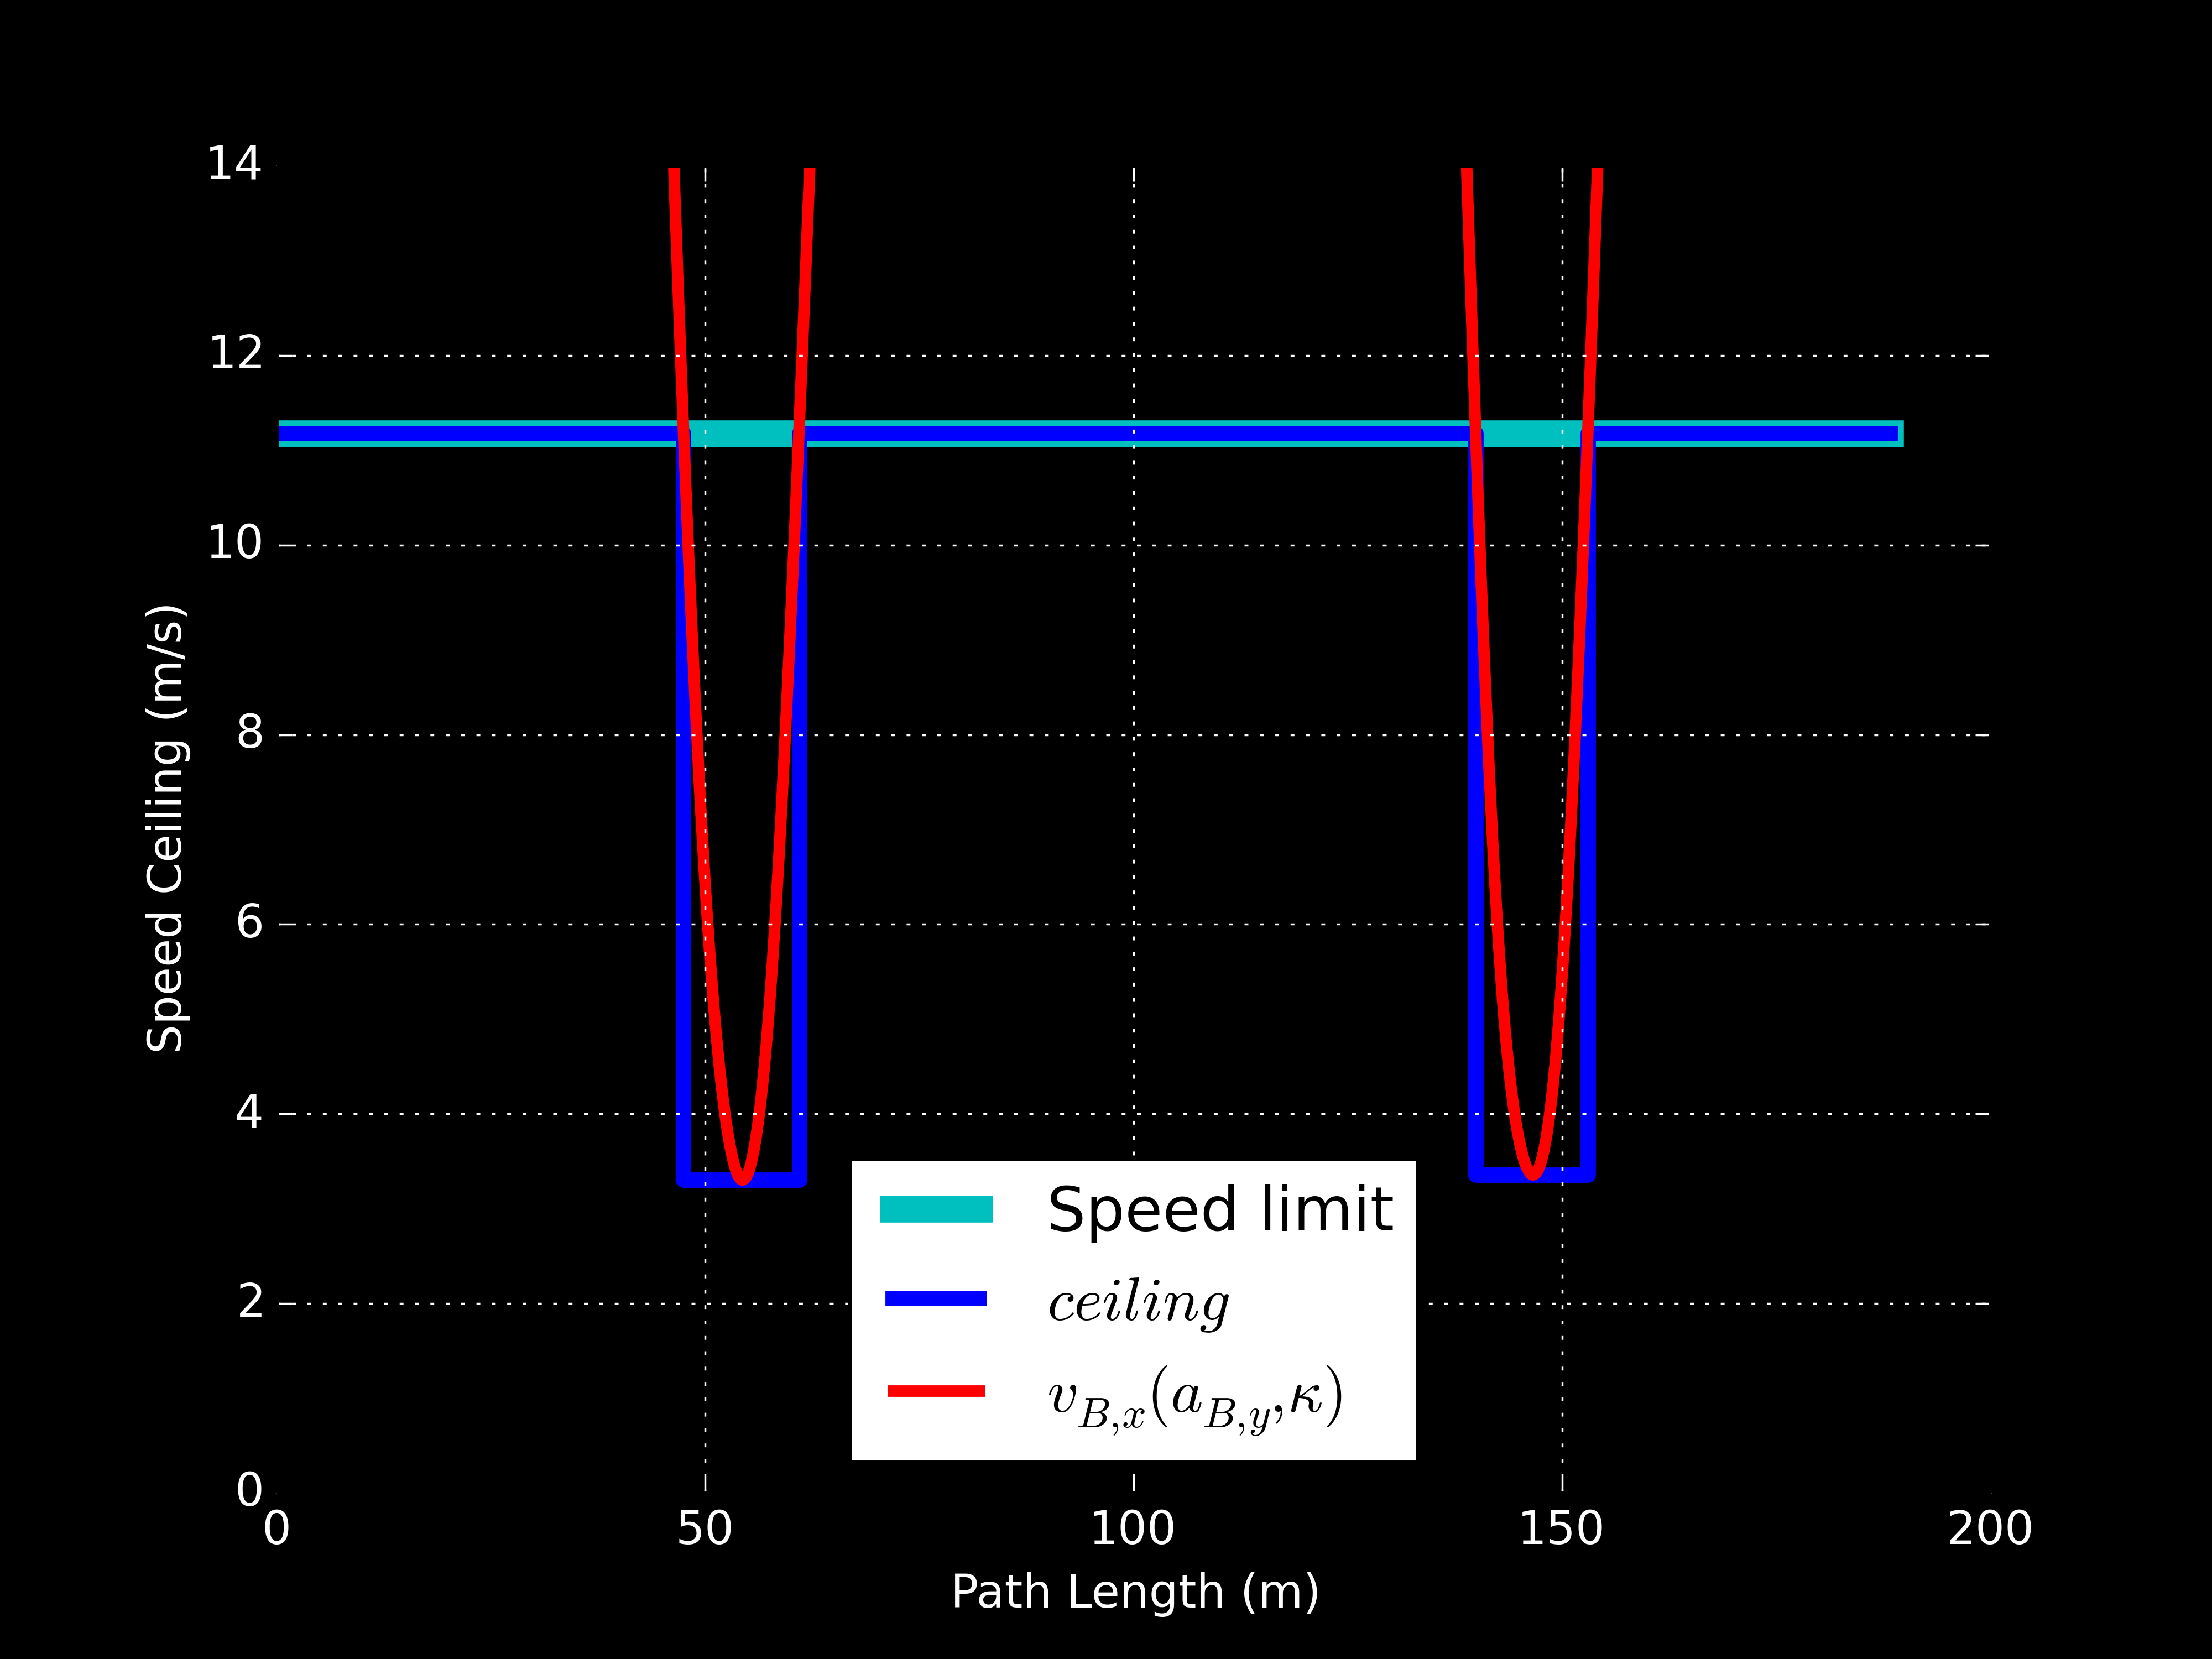
\includegraphics[width=0.8\columnwidth]{graphics/speed_ceiling.png}
  }
  \caption{Dividing a subpath into segments and determining speed ceilings for each segment.}
  \label{fig:1Dto2DandSegmentation}
\end{figure}

% need better notation here.
In the consolidation step, a single set of $\mathbf{b}$, $\mathbf{a}_m$, and $\mathbf{j}_m$ 
%initial/final speeds, speed limit, peak acceleration and jerk 
must be calculated for each segment using the values corresponding to the waypoints comprising the segment.
The minimum of scalar across all constituent points is chosen.
While not time optimal, it ensures that no constraints are violated while still keeping the number of total segments low.
In the present example, this means that in the straight portions of the subpath $v_m = SL$ and in the curves $v_m$ is set to the value required to obtain $a_{B,y}^{max}$ for the entirety of the curve.
As a result, many of the curves will have a constant speed.
For the sake of simplicity, the values of $a^+_{m,k}$, $a^-_{m,k}$, $j^+_{m,k}$, and $j^-_{m,k}$ are initially all set constant for the entire path, using values from \cite{Maurya2012,Hoberock1977,Long2000}.

A jerk vs. time profile is fit to each segment using the algorithm described in the next sub-section.
Speed and acceleration must be continuous between each segment. Only the corresponding speed ceilings have been found, so the start and end conditions for each segment must be determined.
The values of $a_i$ and $v_i$ for the first segment are set to the value currently reported from sensor data.
Since the final acceleration is to be set to zero for all profiles, each subsequent segment may begin with $a_i = 0$.
For the final segment, setting $v_f = 0$ is prudent unless the scenario demands otherwise.
Algorithm~\ref{alg:segmentspeedboundaryconditions} is used to set boundary speed conditions for the interior segments,
with continuity of position, speed, and acceleration.

\begin{figure}
  \begin{algorithmic}[1]
    \Procedure{SegmentBoundarySpeeds}{$v_m$}
      \State $\mathbf{v}_p \gets \mathbf{v}_m$ \Comment{Initialize targets as ceilings}
      \State $\mathbf{v}_{p,0} \gets v_i$ \Comment{Set starting speed to current}
      \State $\mathbf{v}_p = [\mathbf{v}_p, 0]$ \Comment{Add final speed of 0}
      \For{$i = 1, ..., N-1$}
        \If{$v_{m,i+1} > v_{m,i}$}
          \State $v_{p,i+1} \gets v_{m,i+1}$
        \Else
          \State $v_{p,i+1} \gets v_{m,i}$
        \EndIf
      \EndFor
    \EndProcedure
  \end{algorithmic}
  \caption{
    Algorithm to set speed boundary conditions for interior segments.
    Having consolidated the waypoints into a set of path segments, the maximum allowable speed for each segment, $v_{m,i}$ is known.
    This algorithm uses the set of $\mathbf{v_{m}}$ for all segments to choose the highest allowable start and end speeds for each path segment.
    ????????? define $v_p$ ???????????
  }
\label{alg:segmentspeedboundaryconditions}
\end{figure}

Now that all segments within the subpath have been parameterized, they may be solved sequentially.

%%%%%%%%%%%%%%%%%%%%%%%%%%%%%%%%%%%%%%%%%%%%%%%%%%%%%%%%%%%%%%%%%%%%%%%%%%%%%%%%

\subsection{Fitting Jerk Profiles to Each Segment} \label{sec:jerkprofiles}

To introduce the process of computing a jerk profile for each segment, let us consider the case in which a vehicle needs to travel some arbitrary distance ahead.
The vehicle is moving at an initial speed and needs to accelerate to a traveling speed, maintain that speed for some distance, then brake to a stop at a prescribed end location.
Figure \ref{fig:full7phasespec} shows this trajectory over time.

\begin{figure}[tb]
  \centering
  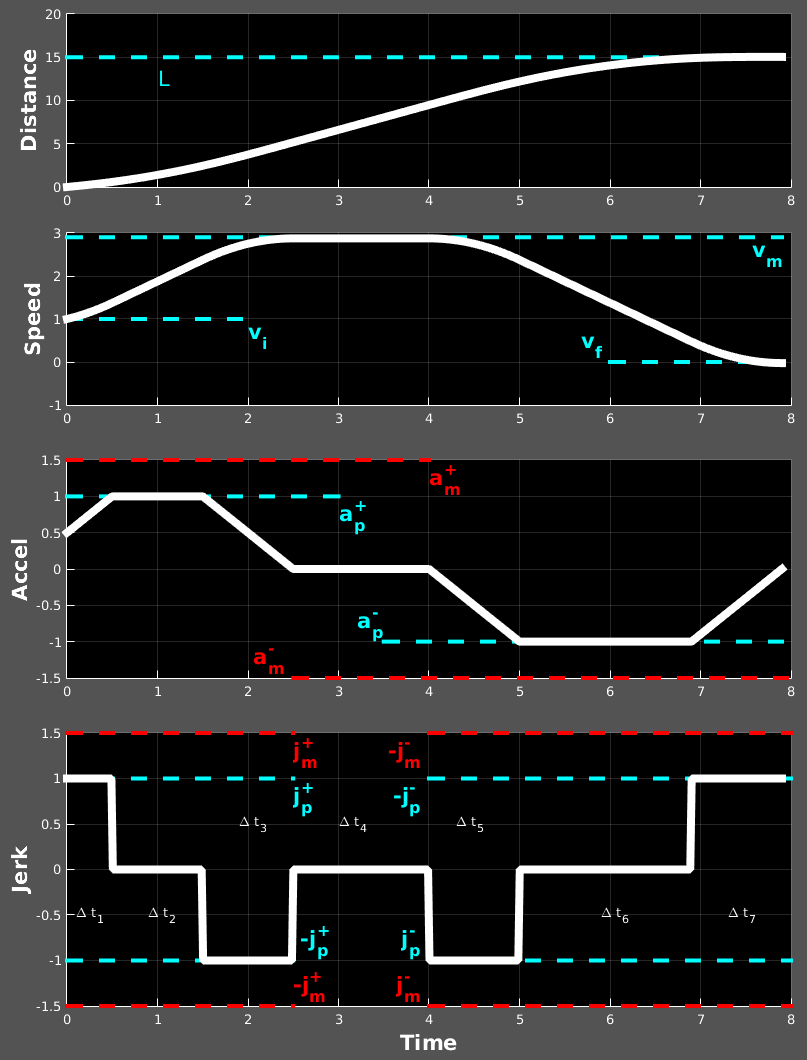
\includegraphics[width=1.0\columnwidth]{graphics/Full7PhaseSpecVertical.png}
  \caption{
    7-phase constant jerk profile along the curvilinear distance axis.
    All values needed to completely parameterize a single path segment for trajectory are labeled here.}
  \label{fig:full7phasespec}
\end{figure}


Final forward acceleration is set to zero.
A profile with $M$ constant jerk phases (7 in this case) can be generated by solving for the time intervals $[\Delta t_1, ..., \Delta t_M]$.
As we show later, $\mathbf{a}_m$, and $\mathbf{j}_m$ must sometimes be modified to obtain physically possible time intervals.
To enable this, ranges of acceptable longitudinal jerk and acceleration $\mathbf{a}^{max}_m = [a^{+,max}_m , a^{-,max}_m]$ and $\mathbf{j}^{max}_m = [j^{+,max}_m , j^{-,max}_m]$ are set according to the relation in Eqs. \ref{eq:am} and \ref{eq:jm}.
In the simplest case, one value for each of the quantities expressed in these relations may be chosen for the entire path.

\begin{equation}
  a^{+,max}_m >= a^+_m > 0 > a^-_m >= a^{-,max}_m
  \label{eq:am}
\end{equation}
\begin{equation}
  j^{+,max}_m >= j^+_m > 0 > j^-_m >= j^{-,max}_m
  \label{eq:jm}
\end{equation}

We propose to define 4 other basic profiles to cover all feasible values in $\mathbf{b}$, and our algorithm judiciously chooses the appropriate profile. These 4 profiles cover cases in which the 7-phase solution fails. For instance, if $L$ is too short or $v_m$ is too high, then it will not be possible to ever reach $v_m$ with realistic values of $\mathbf{a}_m$ and $\mathbf{j}_m$.
%The other profiles are explained below.
All impossible scenarios are automatically ruled out (e.g., end speed above speed limit, traveling speed of zero, negative speeds in $\mathbf{b}$, etc).
It should be noted that traveling backward (i.e., in reverse gear) is not supported in this work.
To find closed-form solutions for $[\Delta t_1, ..., \Delta t_M]$, given $\mathbf{b}$, $\mathbf{a}_m$, and $\mathbf{j}_m$, a symbolic solver is used 
%\textbf{RG: can specify solver name???} .
These 4 profiles are:

\subsubsection{7-phase} \label{sec:7phase}

This profile, with $\Delta t_i$ as shown in Figure \ref{fig:full7phasespec}, is always attempted first.
All time steps have a single solution, enabled by the fact that the initial and end conditions are known, and the two peak accelerations and two jerk magnitudes are provided as configuration parameters.
In the case where $\Delta t_2$ or $\Delta t_6$ are negative, accel-jerk tuning must be employed.
The 7-phase profile can be expressed as $( j_1 > 0 , j_2 = 0 , j_3 < 0 , j_4 = 0 , j_5 < 0 , j_6 = 0 , j_7 > 0 )$.
In the instance where $\Delta t_4$ is negative, the total segment length $L$ is too short to reach top speed of $v_m$, so a 6-phase profile must be used.

\subsubsection{6-phase} \label{sec:6phase}

In the case mentioned above, the speed limit is too high for a solution to exist for a 7-phase profile.
The middle travel period $\Delta t_4$ is removed, so that the vehicle increases speed and then immediately decreases speed. 
The peak speed, in this case, has a solution that cannot be manipulated directly.
Without this known value, the problem becomes under-defined, so $\Delta t_2$ and $\Delta t_5$ each have two solutions: one negative and one positive.
The positive solution is chosen.
In the case where both solutions are negative, accel-jerk tuning is attempted. 
The 6-phase profile can be expressed as $( j_1 > 0 , j_2 = 0 , j_3 < 0 , j_4 < 0 , j_5 = 0 , j_6 > 0 )$
Should that yield no positive time intervals, one of the two 4-phase profiles then becomes appropriate, since $L$ is not large enough to accommodate accelerating past the end speed.
If $v_i > v_f$, then a reversed 4-phase profile is attempted.
However, if $v_i > v_f$, then a regular 4-phase profile is attempted.

\begin{figure}[tb]
  \centering
  \begin{tabular}{cc}
  \subfigure[6-phase profile] {
  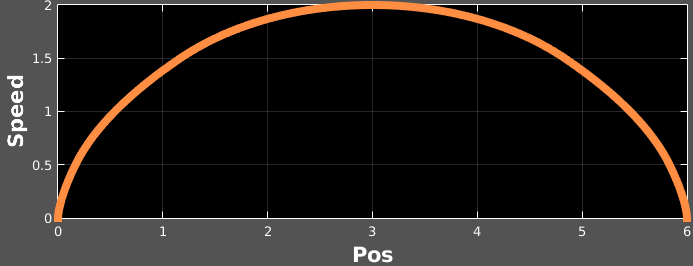
\includegraphics[width=0.43\columnwidth]{graphics/6phase_v(s).png}
  \label{fig:6phaseprofile}
  } &
  \subfigure[4-phase profile] {
  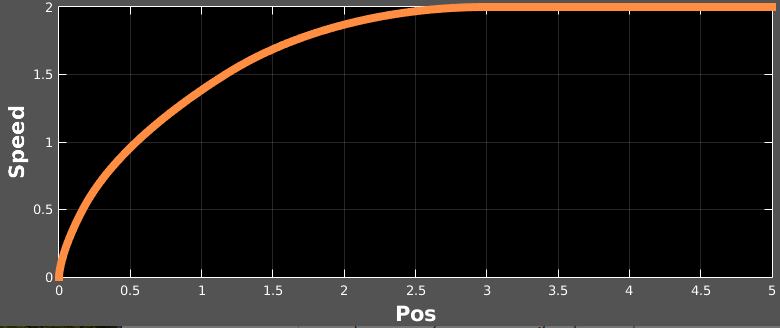
\includegraphics[width=0.43\columnwidth]{graphics/4phase_v(s).png}
  \label{fig:4phaseprofile}
  } \\
  \subfigure[Reversed 4-phase profile] {
  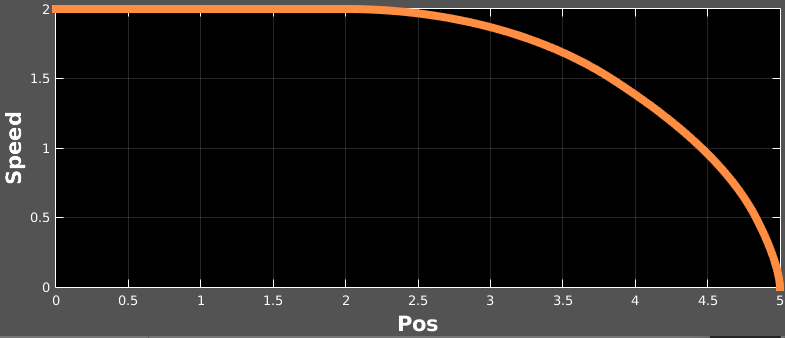
\includegraphics[width=0.43\columnwidth]{graphics/4Rphase_all_derivatives.png}
  \label{fig:4rphaseprofile}
  } &
  \subfigure[3-phase profile] {
  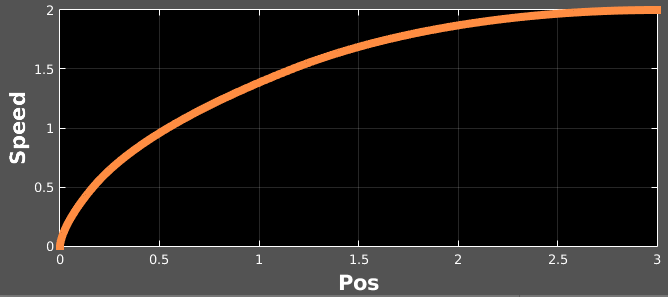
\includegraphics[width=0.43\columnwidth]{graphics/3phase_v(s).png}
  \label{fig:3phaseprofile}
  }
  \end{tabular}
  \caption{6, 4, Reversed 4 and 3-phase profiles, displayed as speed vs. position along path.}

\end{figure}

\subsubsection{4-phase} \label{sec:4phase}

When $v_i < v_m \simeq v_f$, the vehicle should increase speed, then maintain that speed for the distance remaining in the segment.
The 4-phase profile can be expressed as $( j_1 > 0, j_2 = 0 , j_3 < 0, j_4 = 0 )$


\subsubsection{Reversed 4-phase} \label{sec:reversed4phase}

When $v_i \simeq v_m > v_f$, it would be nonsensical to immediately brake.
The initial speed is maintained for a period before applying the brakes.
The reversed 4-phase profile can be expressed as $( j_1 = 0, j_2 < 0, j_3 = 0 , j_4 > 0 )$

\subsubsection{3-phase} \label{sec:3phase}

A change from one speed to another.
All of the above profiles are composed of some combination of a 3 phase profile and a $j = 0$ phase.
This presents a difficulty in that either $L$ or $v_f$ may be enforced, but not both (there is no solution to enforce both).
As such, this profile is chosen only for a segment in which it is impossible to completely arrive at the end speed given the initial conditions.
When these discrepancies in the feasible $v_f$ for a segment arise, the corresponding value in $v_p$ is updated so that the new conditions may be accounted for in the subsequent segment.
The 3-phase profile can be expressed as $(j_1 \pm 0 , j_2 = 0, j_3 \mp 0 )$

% \subsection{Stitching Segment Solutions Together} \label{sec:unifiedsolution}
For each of the profiles, it is possible that the chosen values of $\mathbf{a}_m$ and $\mathbf{j}_m$ will not be feasible for a desired speed at the end of the phase.
This results in a negative time interval for one or more phases.
In many cases, modifying $\mathbf{a}_m$ and $\mathbf{j}_m$ such that they still lie within $\mathbf{a}^{max}_m$ and $\mathbf{j}^{max}_m$ will remedy this.
Specifically, jerk may be increased while peak acceleration is decreased.
This process is referred to herein as ``accel-jerk tuning''.
If no acceptable values are found within the valid ranges of $\mathbf{a}^{max}_m$ and $\mathbf{j}^{max}_m$, a new jerk profile must be chosen.

To decide which profile to employ, a cascade approach is used.
Analytic values of time intervals are evaluated for each profile by plugging in new values of $\mathbf{a}_m$ and $\mathbf{j}_m$ until all time intervals are positive and real.
The order in which they are attempted is: 7 $\rightarrow$ 6 $\rightarrow$ 4 / 4R $\rightarrow$ 3.
Each has been described above.
The routines for fitting a profile to a given $\mathbf{b}, \mathbf{a}_m, \mathbf{j}_m$ to a segment using this cascade approach is referred to as a ``jerk library''.

At this point, the subpath has been divided into segments and an analytically derived plan has been fit to each segment individually.
Now a unified reference trajectory must be constructed by stitching these together.

For each segment with $M$ jerk phases, the following values are computed, which correspond to the instants at which jerk changes:
\begin{itemize}
  \item $M$ time durations $\Delta t_{ref}$. These must be added to the last time value from the previous segment to translate them into reference time.
  \item $M$ jerk values $j(t_{ref})$, which may be appended directly to the preceding jerk values.
\end{itemize}
It is now possible to integrate $j(t)$ to determine an instantaneous trajectory at any moment in time.

% After stitching together control point vectors for time, position, and its derivatives, all information required to have a trajectory plan is now in place.
% To aid in this, univariate splines are created with time as the independent variable, using the control points as knots.
% Position along the path as a function of reference plan time, $s(t)$, takes the form of a cubic Hermite spline, constructed using the speed control points $v_{B,x}(t)$ to set the derivatives.
% Speed along the path $v_{B,x}(t)$ takes the form of a quadratic Hermite spline, with the acceleration control points $a_{B,x}(t)$ used to set the derivatives at every knot.
% Acceleration $a_{B,x}(t)$ is piecewise linear, so lookup is a trivial matter.
% The same applies to $j_{B,x}(t)$, which may be implemented with a simple table.

% However, the time at which the trajectory plan must be referenced is not always known.
% The solution to this problem is known as trajectory tracking control, and will be discussed in Sec. \ref{sec:trajectorytracking}.

%%%%%%%%%%%%%%%%%%%%%%%%%%%%%%%%%%%%%%%%%%%%%%%%%%%%%%%%%%%%%%%%%%%%%%%%%%%%%%%%

\subsection{Reactive Stop Trajectories} \label{sec:reactivestoptrajectory}

The procedure for planning NORMAL mode trajectories is separate from that used to compute RSTOP trajectories.
For RSTOP trajectory, a 3-phase profile is used, with end conditions $v_f=0, a_f=0$ and initial conditions set to the current state of the navigation filter.
While it would seem that the 3-phase segment solving procedure described in Sec. 
%\ref{sec:3phase} 
\ref{sec:jerkprofiles} can be applied to reactive stopping, this is not the case.
As was mentioned previously, only one of $[L, v_f]$ may be rigidly enforced for a 3-phase profile, but not both, since no closed-form solution exists for that case.
Normal planning enforces $L$ to avoid skewing segment boundaries within each subpath.
However, reactive stopping requires that $v_f$ be enforced, and that we solve for $L$.
Reformulating a new 3-phase jerk profile accordingly is a simple matter for the symbolic solver.
%%% This is the brief way of wording the preceding three sentences.
% The trajectory planner uses total distance as parameter, and is not suitable for our purpose as the end speed constraints are not met. So we reformulate and replace $L$ with $v_f$ as the hard constraint.

Now appropriate values of $a_m^-$ and $j_m^-$ must be chosen to completely parameterize the trajectory.
For calculating $\Delta s_{RSTOP}$, the same set of values from normal planning is used and the distance traversed in the resultant trajectory is reported as the current value of $\Delta s_{RSTOP}$.

Once the path manager triggers RSTOP, the trajectory is then recomputed with increasingly higher absolute values of $a_m^-$ and $j_m^-$ until $\Delta s_{RSTOP} <= \Delta s_{avail}$.
Should one of the values $a_m^-$ or $j_m^-$ required to fulfill this condition exceed the limits $a_m^{-,max}$ or $j_m^{-,max}$, then limit braking parameters are set such that $a_m^-=a_m^{-,max}$ and $j_m^-=j_m^{-,max}$, and the user is alerted.

% After this, the spline creation procedure detailed in Sec. \ref{sec:unifiedsolution} is performed.
The path must now be truncated for 1D $\leftrightarrow$ 2D transformation.
Within the trajectory tracker, all portions of the path leading up to the location of RSTOP triggering are removed, as well as the portions after the location which corresponds to $s_{veh} + \Delta s_{RSTOP}$.
% This is depicted in Fig. \ref{fig:pathtostop}
The vehicle now begins sampling from this trajectory and executes a smooth reactive stop.

%\begin{figure}[thpb]
%  \centering
%  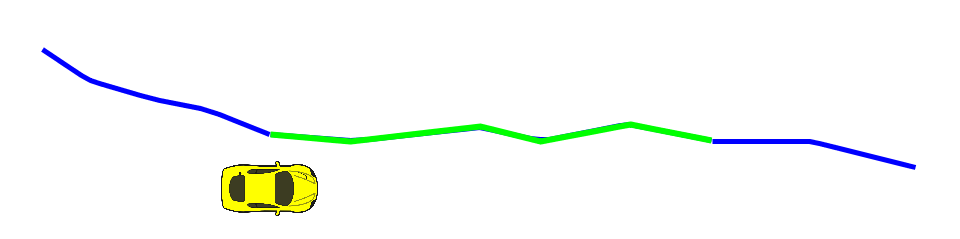
\includegraphics[width=1.0\columnwidth]{graphics/RSTOP_path_truncation.png}
%  \caption{Green color path is the one over which the car finds a trajectory to stop. please show green as dashes for b\&w printing ??????????? }
%  \label{fig:pathtostop}
%\end{figure}

However, the time at which the trajectory plan must be referenced is not always known.
The solution to this problem is known as trajectory tracking, and will be discussed in the next section.


%%%%%%%%%%%%%%%%%%%%%%%%%%%%%%%%%%%%%%%%%%%%%%%%%%%%%%%%%%%%%%%%%%%%%%%%%%%%%%%%
%%%%%%%%%%%%%%%%%%%%%%%%%%%%%%%%%%%%%%%%%%%%%%%%%%%%%%%%%%%%%%%%%%%%%%%%%%%%%%%%

\section{Trajectory Tracking} \label{sec:trajectorytracking}

After planning has been performed, a reference signal must be regularly supplied to the control system in order for the vehicle to carry out the plan.
%This is known as tracking.
The primary difficulty here is that the trajectory plan has been developed in a 1D position space using a reference time which has an unknown drift relative to real time.
As such, we must find a way to look up the coordinates of the vehicle within the reference trajectory using information typically available for autonomous cars.
A minimal set of such information includes position, velocity vector, heading, and acceleration in the body frame.
It is assumed that the vehicle controller will need samples of a small window into the future trajectory to pilot the vehicle.

\begin{figure}[thpb]
  \centering
  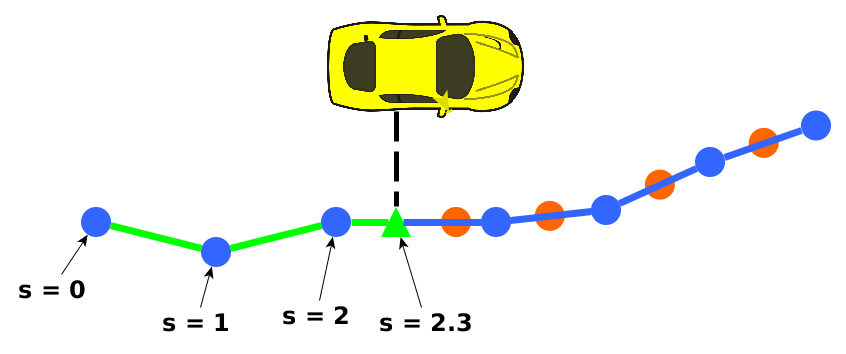
\includegraphics[width=0.8\columnwidth]{graphics/PathProjectionSlice.png}
  \caption{Showing projection of the current position of the car shown by green triangle to s coordinate system. Each circle represents a node, and the lines between them are links. The orange dots indicate future trajectory samples which are sent to the controller.
  }

  \label{fig:cartos}
\end{figure}

The general idea is to project the vehicle's current position onto the path, and then find the cumulative distance along the path between the start point and the projection point.
The 2D vehicle position is thus transformed into a 1D location corresponding to the vehicle's current reference time.
Once this reference time is obtained, it may be used to look up position, speed, acceleration, and jerk along the curve of the path over the future time window.
From there it is a matter of simple geometry to transform these values into the coordinate system of the path and, subsequently, any other coordinate system which may be needed.

% \subsection{Path Projection} \label{sec:pathprojection}

Several algorithms exist to find the optimal projection of the target vehicle's present kinematic state (position, velocity and acceleration vectors) onto the path.
A simple approximation is to perpendicularly project the vehicle's position onto a series of lines running between each pair of adjacent points in the path (this will be referred to as a ``link'', and is depicted in Fig. \ref{fig:cartos}).
Projections which lie outside of the link's two constituent path points are snapped to the nearest one.
The projection which is closest to the vehicle's actual position is then assumed to be the correct path projection $\mathbf{r}_p$.
Any number of modifications can be made using heading, velocity vectors, and previous information to allow this method to be extended to complex overlapping paths or self-intersections.

Choice of an algorithm to obtain the current 1D position of the vehicle along the length of the path $s_{veh}$ (i.e., in the same 1D $s$-coordinate system in which the planning was performed) is influenced by the form of the path plan.
We assume that the path is linear between waypoints to significantly reduce the computational effort.
So $s_{veh}$ at any epoch is the sum of the link lengths behind its perpendicular projection $\mathbf{r}_p$.
However, the error in this approximation approaches zero as the spacing between path points approaches zero.
Other, more accurate, approximations which work well include cubic splines, arc splines, and Bezier curves, which have solutions for closest point projection and arc-length calculation~\cite{Wang2002,Wang2003,Schindler2011}.

Now the reference time corresponding to the vehicle's location $t_{veh}$ is needed to look up $v_{B,x}(t_{veh})$, $a_{B,x}(t_{veh})$, and $j_{B,x}(t_{veh})$.
Additionally, it is also needed to sample $s(t)$ at intervals ahead of the vehicle.
Since it is known that $s(t)$ is piecewise cubic, reference time as a function of vehicle position along the path, $t(s)$, may be approximated as cubic using a spline.
To get the knots, $s(t)$ is sampled at $\Delta t = 0.01 sec$.
This yields two vectors $s'$ and $t'$ which are then used to create a univariate cubic $t(s)$ spline.
Evaluating $t(s_{veh})$ then yields the current reference time.

%%%%%%%%%%%%%%%%%%%%%%%%%%%%%%%%%%%%%%%%%%%%%%%%%%%%%%%%%%%%%%%%%%%%%%%%%%%%%%%%
%%%%%%%%%%%%%%%%%%%%%%%%%%%%%%%%%%%%%%%%%%%%%%%%%%%%%%%%%%%%%%%%%%%%%%%%%%%%%%%%

To summarize, in the last three sections we described how an urban path is broken into sub-paths. We 
explained the computation of velocity and jerk profile for segments within sub-paths that honor constraints
for speed, velocity and acceleration as well as reactively slow down or stop for pedestrians on
the urban path. We then described how our trajectory plan is supplied regularly in real-time to the
autonomous car controller.

\section{Summary} \label{sec:summary}


In this paper, we have presented a novel real-time method for planning longitudinal trajectories 
in an autonomous car to follow an urban path with online updates to avoid pedestrians on the roadway by slowing down or 
stopping.
We built a robust stopping model as part of Trajectory Planner reliably integrated with the Path Manager.
We can travel along a desired path, stop at stop signs, stop for pedestrians in the roadway, and continue after 
they leave. Our system gracefully handles complex cases that were not explicitly programmed, such as following 
pedestrians if they continue walking on the road away from the car. Our system works with multiple 
pedestrians as we only need to consider the closest pedestrian ahead of us. 

\textbf{emphasize limited knowledge of pedestrians as a strength}

We make three contributions in this paper. First, we present an integrated trajectory planner that
simultaneously limits jerk, velocity and acceleration to pre-set desired values while being responsive 
to the presence of pedestrians.
Second, our trajectory planner has closed form solution and is suitable for online implementation
on a car, unlike systems requiring solutions to nonlinear optimizations. Finally, we have confirmed the
efficiency and reliability of our trajectory planner on a test vehicle with over 100 hours of testing
under fully autonomous driving conditions on urban roads with pedestrians in random locations. 

In future, we would like to handle other roadway traffic, perceiving and reacting to other vehicles. We would also like to perceive and stop for stop signs and red-lights,
rather than using map information.


%%%%%%%%%%%%%%%%%%%%%%%%%%%%%%%%%%%%%%%%%%%%%%%%%%%%%%%%%%%%%%%%%%%%%%%%%%%%%%%%
%%%%%%%%%%%%%%%%%%%%%%%%%%%%%%%%%%%%%%%%%%%%%%%%%%%%%%%%%%%%%%%%%%%%%%%%%%%%%%%%
%%%%%%%%%%%%%%%%%%%%%%%%%%%%%%%%%%%%%%%%%%%%%%%%%%%%%%%%%%%%%%%%%%%%%%%%%%%%%%%%

\bibliographystyle{IEEEtran}
\bibliography{root}

\end{document}
